% PCT-SOURCE: pdf=200 print=188 kind=figure id=A.2
% Native reconstruction of the Ising phase diagram on source page 188.
\begingroup
\renewcommand{\thefigure}{A.2}
\renewcommand{\figurename}{Figure}
\begin{figure}[htbp]
  \centering
  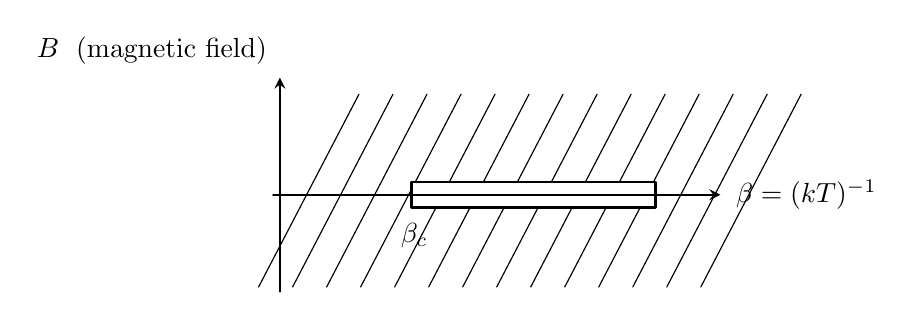
\begin{tikzpicture}[x=1.08cm,y=.96cm,>=stealth,line cap=round,
    line join=round]
    % Diagonal hatching marks the two-phase line's surrounding phase
    % diagram.  The white strip is the B=0 part for beta >= beta_c.
    \foreach \x in {-.25,.15,.55,.95,1.35,1.75,2.15,2.55,2.95,3.35,3.75,4.15,4.55,4.95}
      \draw[line width=.42pt] (\x,-1.22) -- ++(1.18,2.55);

    \draw[->,line width=.75pt] (0,-1.28) -- (0,1.55)
      node[above left=1pt] {$B$\; (magnetic field)};
    \draw[->,line width=.75pt] (-.08,0) -- (5.18,0)
      node[right=2pt] {$\beta=(kT)^{-1}$};

    % The critical half-line lies on B=0.  Its outlined strip preserves the
    % double ruled line visible in the scan.
    \fill[white] (1.55,-.17) rectangle (4.42,.17);
    \draw[line width=.9pt] (1.55,-.17) rectangle (4.42,.17);
    \draw[line width=.55pt] (1.55,0) -- (4.42,0);
    \node[below=2pt] at (1.58,-.17) {$\beta_c$};
  \end{tikzpicture}
  \caption{Phase diagram of the Ising ferromagnet (nearest-neighbor interaction). The phase is unique and the correlation functions decay exponentially for all values of $\beta$ and $B$ except those satisfying $B=0$, $\beta_c\leq\beta<\infty$, where there are exactly two phases. The phase diagram for the $\lambda\varphi^4+\mu\varphi^2+\nu\varphi$ model is similar, with $B$ replaced by $\nu$ and $\beta$ by $\lambda$. The solution is known to be unique for $\nu\ne0$ and for all sufficiently small positive $\lambda$. It is known that at least two solutions, I and II, exist for all sufficiently large $\lambda$ with $\varphi\to-\varphi$ symmetry broken in the sense that $\matrixel{\Omega_{0I}}{\varphi_1(x)}{\Omega_{0I}}=-\matrixel{\Omega_{0II}}{\varphi_1(x)}{\Omega_{0II}}\ne0$.}
  \label{fig:A-2}
\end{figure}
\endgroup
